% This must be in the first 5 lines to tell arXiv to use pdfLaTeX, which is strongly recommended.
\pdfoutput=1
% In particular, the hyperref package requires pdfLaTeX in order to break URLs across lines.

\documentclass[11pt]{article}

% Remove the "review" option to generate the final version.
\usepackage[]{ACL2023}

% Standard package includes
\usepackage{times}
\usepackage{latexsym}
\usepackage{graphicx} 
\usepackage{float}
\usepackage{caption}
\usepackage{cuted}
\usepackage{subcaption}
\usepackage{amsmath}
\usepackage{amsfonts}

% For proper rendering and hyphenation of words containing Latin characters (including in bib files)
\usepackage[T1]{fontenc}
% For Vietnamese characters
% \usepackage[T5]{fontenc}
% See https://www.latex-project.org/help/documentation/encguide.pdf for other character sets

% This assumes your files are encoded as UTF8
\usepackage[utf8]{inputenc}

% This is not strictly necessary, and may be commented out.
% However, it will improve the layout of the manuscript,
% and will typically save some space.
\usepackage{microtype}

% This is also not strictly necessary, and may be commented out.
% However, it will improve the aesthetics of text in
% the typewriter font.
\usepackage{inconsolata}


% If the title and author information does not fit in the area allocated, uncomment the following
%
%\setlength\titlebox{<dim>}
%
% and set <dim> to something 5cm or larger.

\title{EICQE: Expert Independent Critical Question Evaluation}


\author{
  Rico Staedeli \and Cédric Bohni \\
  University of St. Gallen \\
  \{rico.staedeli, cedricdominique.bohni\}@students.unisg.ch \\ \\
 \textbf{GitHub:} \href{https://github.com/RicoStaedeli/NLP2025_CQG}{\text{https://github.com/RicoStaedeli/NLP2025\_CQG}}
}

\begin{document}
\pagestyle{plain}

\maketitle
\begin{abstract}
The development of Large Language Models (LLMs) has led to impressive performance in mitigation strategies against misinformation, such as counterargument generation. However, LLMs are still significantly limited by outdated knowledge and a tendency to produce hallucinated content. To address these issues, \citet{calvo_figueras_critical_2024} proposed the shared task of \textit{Critical Questions Generation}. This task involves processing an argumentative text to generate the \textit{critical questions} (CQs) it raises. In argumentation theory, CQs are tools intended to expose the blind spots of an argument by highlighting potentially missing information. In this paper, we introduce \textbf{EICQE}, a novel framework for \emph{Expert-Independent Critical Question Evaluation}. Our approach employs a rule-based evaluation system grounded in four argumentation schemes proposed by \citet{walton_argumentation_2008}. Leveraging this evaluation pipeline, we generated two qualitatively annotated datasets: an instruction dataset for supervised fine-tuning and a preference dataset for reinforcement learning. Using these resources, we fine-tuned an LLM with different training approaches and assessed its performance using both the official evaluation script from the shared task and our enhanced EICQE pipeline. Experimental results indicate that the fine-tuned model significantly outperforms the original baseline prior to training, achieving an improvement of over $200\%$ in terms of criticality and alignment with argumentation schemes.
\end{abstract}

\section{Introduction}
Generating valid and insightful critical questions remains a persistent challenge for contemporary large language models (LLMs), particularly when such questions must meaningfully engage with complex argumentative texts. The EICQE framework proposed in this paper contributes to the Shared Task on Critical Question Generation\footnote{\url{https://hitz-zentroa.github.io/shared-task-critical-questions-generation/}}, which aims to foster the development of systems capable of promoting critical thinking through automated question generation. The task is based on the foundational work by \citet{calvo_figueras_critical_2024}, who introduced the problem and associated challenges in their paper \emph{Critical Question Generation: Motivation and Challenges}. They created a small gold-standard dataset comprising critical questions for 186 argumentative texts, using the pre-annotated debate datasets US2016 and Moral Maze. These datasets are annotated according to Walton's argumentation schemes, providing a structured basis for identifying relevant critical questions. The authors generated candidate questions using various LLMs and applied manual filtering based on several evaluation criteria to curate a high-quality reference set \citep{calvo_figueras_critical_2024}. The approach in this paper advances this previous work by introducing an automated evaluation pipeline that eliminates the dependency on expert judgment. This generalization enables broader applicability of the system, particularly during the evaluation phase of fine-tuning LLMs. To reduce the inherent subjectivity of expert-based evaluation, the methodology is based on Walton's argumentation schemes \citep{walton_argumentation_2008}, leveraging their structure and associated critical questions as a theoretical foundation. To generate critical questions, multiple fine-tuning strategies were explored, including supervised fine-tuning (SFT) and Reinforcement Learning techniques. For Reinforcement learning (RL), Direct Preference Optimization (DPO) and Odds Ratio Preference Optimization (ORPO) were employed. 

This paper presents a foundational step toward the development of models that support critical engagement with argumentative content and establishes the groundwork for future research at the intersection of computational argumentation and natural language generation. 
 \newpage 
\begin{strip}
    \centering
    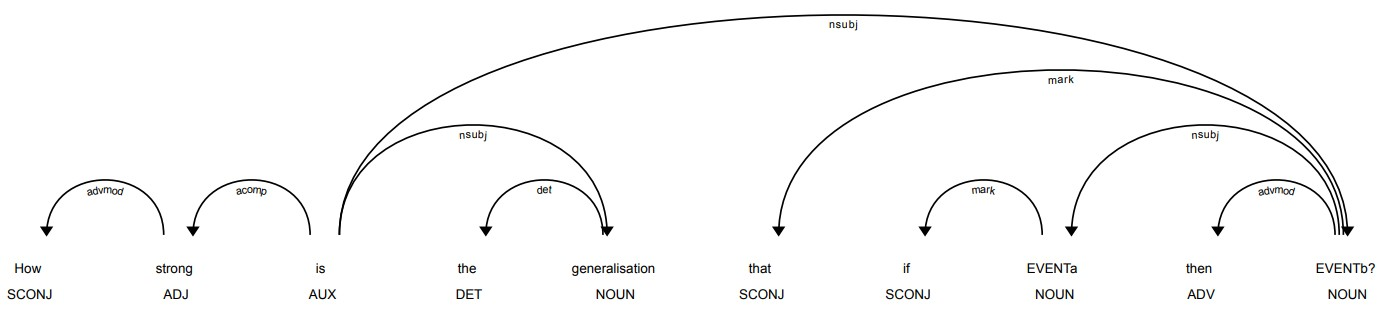
\includegraphics[width=\linewidth]{images/cause_to_effect_cq_tree.jpg}
    \captionof{figure}{Dependency tree of a critical question from the \textit{Cause to Effect} scheme}
    \label{fig:cq-dependency-strength}
\end{strip}

\section{Method}
A key challenge in the Critical Question Generation task is defining what constitutes a valid critical question and how to evaluate whether a question generated by a large language model fulfills that function.  Calvo Figueras and Agerri \cite{calvo_figueras_critical_2024} address this by introducing a framework that operationalizes critical questions through the instantiation of templates derived from Walton's argumentation theory. Building on this approach, we adopted a rule-based methodology to define and implement critical questions, focusing on four representative argumentation schemes: \textit{Cause to Effect}, \textit{Analogy}, \textit{Expert Opinion}, and \textit{Fear-Appeal}. These schemes were selected based on their prevalence and structural clarity in the annotated datasets used in the challenge.

The critical question generation system was implemented as a rule-based pipeline tailored to these four schemes. We used \texttt{spaCy} for dependency parsing and part-of-speech tagging, \texttt{WordNet} to leverage semantic relations, and \texttt{FrameNet} to identify event frames. This combination enabled the extraction of key argument components and the instantiation of template-based critical questions for each scheme.

In our implementation, dependency parsing facilitated the identification of syntactic structures corresponding to the components of Walton's argumentation schemes. For example, causal relations in the \textit{Cause to Effect} scheme were detected through subordinating conjunctions like "because" or "if," while comparative constructions in the \textit{Analogy} scheme were identified using phrases such as "like" or "similar to." By mapping these linguistic cues to the respective argumentation schemes, our system effectively generated critical questions that align with the theoretical underpinnings of Walton's framework.

Recent research in the field underscores the efficacy of classical linguistic tools such as dependency parsing in modeling and extracting argumentative structures. Ye and Teufel \cite{ye-teufel-2021-end} propose a neural end-to-end approach to argument mining by framing it as a dependency parsing problem. Their argument mining dependency parser outperforms previous state-of-the-art models, achieving F1 scores of 73.5\% for component identification and 46.4\% for relation identification. This work highlights the potential of dependency parsing in argument mining that captures the structure of arguments. Their approach led us to the idea that similar argument structures for critical questions can be modeled as dependency graphs, where components such as causes, claims, analogs, or expert attributions are connected through identifiable syntactic or structural patterns. We build on their assumption that dependency parsing can extract meaningful relations and want to make use of rule-based pattern matching to model Walton's critical question templates. 


\subsection{Rule-based heuristics}

\noindent
As an example, we look at Figure \ref{fig:cq-dependency-strength} illustrating the syntactic structure of a critical question from Walton’s \textit{Cause to Effect} scheme. The sentence consists of a main interrogative clause and an embedded conditional clause. 
The \textbf{main clause} (“How strong is the generalisation”)
introduces the evaluative frame, linking \textit{is} to the subject \textit{generalisation} (via \texttt{nsubj}) and its property \textit{strong} (via \texttt{acomp}). The modifier \textit{How} is attached as \texttt{advmod}, indicating a degree question.

The \textbf{embedded clause} (“that if EVENTa then EVENTb”) encodes the causal relationship. The subordinating conjunction \textit{if} is labeled \texttt{mark}, while \textit{then} serves as an \texttt{advmod} indicating a consequence. The nominal phrases \textit{EVENTa} and \textit{EVENTb} appear as \texttt{nsubj}, reflecting subject roles in their respective clauses. These syntactic dependencies reflect the logical pattern of the \textit{Cause to Effect} scheme. 
In our implementation, detecting this combination of features, especially \texttt{mark}, \texttt{advmod}, and multiple \texttt{nsubj} relations, serves as a syntactic-level indication that a sentence expresses causal reasoning. These structural cues contribute to the rule-based scoring system, which is further supported by lexical-semantic resources such as \texttt{WordNet} and  \texttt{FrameNet} to verify and reinforce the presence of argumentation patterns. This combined validation allows the system to instantiate appropriate critical questions in line with the templates defined by Walton.

\begin{table}[H]
    \centering
    \begin{tabular}{p{1.2cm}llp{2.5cm}}
        \hline
        \textbf{Token} & \textbf{POS} & \textbf{Dep} & \textbf{Function in Argument} \\
        \hline
        How              & SCONJ   & advmod     & Degree modifier \\
        strong           & ADJ     & acomp      & Adjective complement \\
        is               & AUX     & ROOT       & Main verb (copula) \\
        general-isation   & NOUN    & nsubj      & Subject (main clause) \\
        that             & SCONJ   & nsubj      & Complementizer \\
        if               & SCONJ   & mark       & Conditional clause marking \\
        EVENTa           & NOUN    & nsubj      & Subject of cause \\
        then             & ADV     & advmod     & Temporal/modal marker \\
        EVENTb           & NOUN    & nsubj      & Subject of effect \\
        \hline
    \end{tabular}
    \caption{\label{tab:cause-effect-dependencies}
    Dependency roles in the critical question “How strong is the generalisation that if EVENTa then EVENTb?”
    }
\end{table}

\subsection{Evaluation System}
\label{evaluation system section}
The rule-based heuristic and lexical semantic occurrence approach is then used to evaluate questions on their degree of fulfillment of a schema. For this, we use our scoring system, which measures how strongly a question aligns with a given schema. As introduced, each schema consists of different criteria and, if met, provides scores from 0.5 to 3 depending on its relevance. A question can have a total score of 0 to 10. After analyzing the scoring and balancing the weights, we established that a question with a score of at least 4 indicates a match with the schema, but not sufficient for it to be deemed critical. To ensure that we do not misclassify the questions, we further strengthened the threshold to at least 7 points for a question to be labeled as critical.

To fully evaluate a question, we have designed a three-step approach. We first verify that a text is a question and does not consist of random word repetitions, which would jeopardize the scoring system. After that, the scoring system is used to assess whether the question is critical according to the schema. Lastly, we look at the semantics of the question. In alignment with the established evaluation of the use of cosine similarity in essay assessments, we found it sufficient to use cosine similarity for our evaluation in alignment with the context \cite{lahitani2016cosine}. Following existing research, we are also considering a threshold of 0.5 to determine if there is a semantic similarity \cite{koudas2004flexible}.

To complete the evaluation, we include the original evaluation of the Shared Task on Critical Question Generation\footnote{\url{https://hitz-zentroa.github.io/shared-task-critical-questions-generation/}}. In this evaluation, it compares the generated question to pre-selected questions from each context and assigns labels based on the closest pre-selected question it aligns with. The labels contain 'Useful', 'Unhelpful', and 'Invalid', where 'Useful' indicates a critical question. The preselected questions were given in the provided validation set. The validation set is the largest data set of the original task, so we retrofitted it as a test set, allowing comparison with other models. The determination of closeness was introduced using two different approaches: cosine similarity or Bleurt. In our early trials with the original dataset, we found that a 0.5 threshold cosine similarity is a more reliable metric. Bleurt had too strong punishments, and closeness was nearly never the case, despite significant alignment in cosine similarity.

\subsection{Dataset Generation}
In their work \textit{Critical Question Generation: Motivation and Challenges}, \citet{calvo_figueras_critical_2024} introduce a gold-standard dataset of critical questions aligned with argumentative texts~\citep{calvo_figueras_critical_2024}. The texts in their dataset are predominantly situated within political contexts. Their final publicly available dataset includes annotated questions for 297 argumentative contexts drawn from the US2016 dataset \citep{visser_argumentation_2020}, as well as 73 contexts from the Moral Maze corpus~\citep{lawrence-reed-2015-combining}. We used this dataset for validation purposes in our study. The objective of our work is to develop a system capable of generating more universal and evidence-based critical questions. To this end, we fine-tune a large-language model (LLM) on additional data to enhance its generalization capability. Given that the fine-tuning strategies employed require datasets with varying structures, we began by surveying existing large-scale question generation corpora. Specifically, we examine:
\begin{itemize}
    \item \textbf{HotpotQA}, a dataset designed for diverse, explainable multi-hop question answering \citep{yang_hotpotqa_2018},
    \item \textbf{TriviaQA}, a large-scale QA dataset containing approximately 650k question--answer pairs \citep{joshi_triviaqa_2017},
    \item \textbf{SocratiQ}, a corpus of around 110k context--question pairs, developed to support context-based question generation \citep{ang_socratic_2023}.
\end{itemize}
Our review of the literature revealed a critical gap: no existing dataset is explicitly designed for the task of \textit{critical} question generation. This gap may be attributed to the lack of a precise and operationalized definition of what constitutes a critical question. The HotpotQA and TriviaQA datasets are not well aligned with the task of generating critical questions (CQ), as their primary focus is on identifying correct answers to predefined questions. In contrast, the SocratiQ dataset is somewhat more suitable for our task, as it is designed to evaluate the question-generation capabilities of modern LLMs.  An excerpt of the SocratiQ dataset can be found in table \ref{tab:Excerpt of SocratiQ dataset}. 
\begin{table} [ht]
\centering
\begin{tabular}{p{3cm}p{4cm}}
\hline
\textbf{Input} & \textbf{Target (Question)} \\
\hline
I'm referring only to aesthetics. & Are they obligated to make clothes that are as beautiful as possible? \\
\hline
If you are genuinely struggling and need help, someone is going to want to help you. & How old are the kids who are screaming in public? \\
\hline
\end{tabular}
\caption{Examples entry from SocratiQ dataset.}
\label{tab:Excerpt of SocratiQ dataset}
\end{table} 
Despite SocratiQ providing a diverse dataset of questions, not all can be used in our training. This originates from our reduced schema diversity, which does not cover all possible question types. Since we only took four schemas into account, we filtered the dataset by extracting the questions that align with our defined criteria and have at least one schema as critical ($\geq 7$). This preemptively reduces confusion with other schemes that were not considered in our current development stage.
\begin{table}[ht]
    \centering
    \begin{tabular}{p{0.7cm}p{1.4cm}p{1.1cm}p{1.4cm}p{1.3cm}}
        \hline
        \textbf{Score} & \textbf{Cause to Effect} & \textbf{Analogy} & \textbf{Expert Opinion} & \textbf{Fear-Appeal} \\
        \hline
        0.0 & 45081 & 4466 & 49444 & 650 \\
        1.0 &358 &3178  &2423 & 32 \\
        2.0 & 15451 & 15157& 12691& 55079 \\
        3.0& 1093 &27914  &7266 & 11209 \\
        3.5  &4427 &9877 &  83  &0 \\
        \hline
        4.0 & 5360 & 6202 & 5037 & 8837 \\
        4.5   & 1205 & 3193 & 43 & 0 \\
        5.0  & 5020 & 807  & 1915 & 3845 \\
        5.5  & 844 & 482 & 19  & 0 \\
        6.0  & 642  & 1758 &  620& 745 \\
        6.5   & 212 & 732 & 6  & 0 \\
        \hline
        7.0   &  70 & 686 &  208 &  433 \\
        7.5  & 26 & 362  &  4  & 0 \\
        8.5  & 588 & 49  & 1 & 0 \\
        9.0  & 488 & 6  & 6  & 28 \\
        9.5 & 116 &  2 & 0 & 0 \\
        10.0  & 4 & 1  &  0  & 2 \\
        \hline
    \end{tabular}
    \caption{Scores of SocratiQ}
\end{table} 
This filtering was guided by the evaluation and scoring framework we developed, as detailed in Section \ref{evaluation system section}. We now have a dataset only with questions marked as critical during the evaluation. The dataset used for supervised fine-tuning (SFT) is structured with four columns. The first column contains a unique identifier for each entry, followed by the context, the corresponding question, and finally the highest scoring schema associated with that question. In contrast, the dataset used for Direct Preference Optimization (DPO) fine-tuning follows a different format, consisting of three columns. The first column includes the prompt, which combines the context with the instruction given to the language model. The second column contains the \textit{chosen} response, while the third column provides the \textit{rejected} response for the same prompt. This format facilitates preference-based training by encouraging the model to distinguish and prioritize preferred responses, drawing on reinforcement learning principles without the need for explicit reward signals \citep{rafailov_direct_2024}. To construct the DPO dataset, we developed an automated pipeline designed to generate a rejected question for a given context. The pipeline builds upon the filtered version of the SFT dataset, which includes only context--question pairs identified as relevant CQs. For each context, a new question is generated that targets the most prominent schema underlying the original question. This question generation is performed using the OpenAI API with the \texttt{gpt-3.5-turbo} model. The resulting question is then evaluated using the previously introduced scoring framework. If the generated question falls below the defined threshold for classification as a critical question, it is labeled as a ``rejected'' example for that context. This process is illustrated in Figure \ref{fig:dpo pipeline}.

\begin{figure}[H]
    \centering
    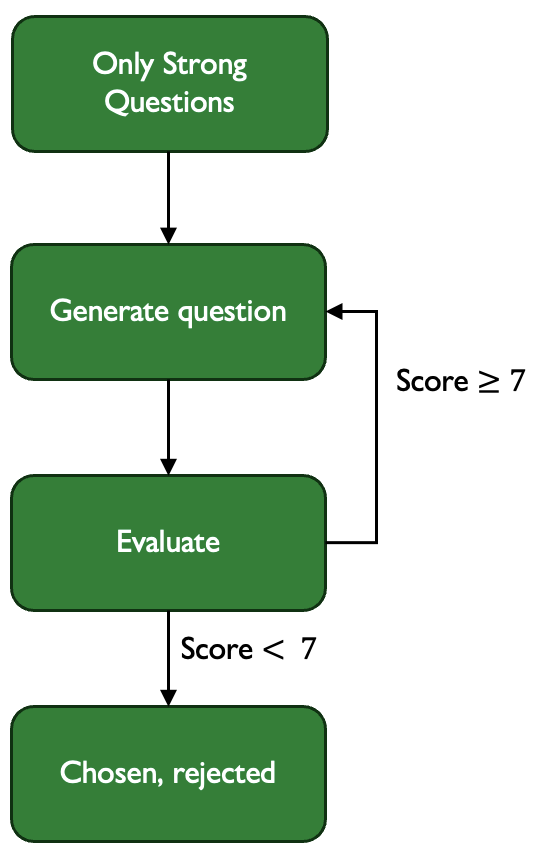
\includegraphics[width=0.25\textwidth]{images/DPO dataset generation.png}
    \caption{DPO Dataset generation pipeline}
    \label{fig:dpo pipeline}
\end{figure}
This generation process results in a new dataset specifically tailored for use in Direct Preference Optimization (DPO) training. By systematically generating and scoring alternative questions, the pipeline distinguishes between high-quality critical questions and those that do not meet the threshold, thereby enabling the construction of preference pairs. These pairs consist of a preferred (accepted) and a less preferred (rejected) question for the same context, which are essential for effective DPO supervision. The outcome of this data preprocessing step is the creation of two distinct datasets: one containing accepted critical questions and the other containing their corresponding rejected counterparts. The statistics of these datasets are summarized in Table \ref{tab:stats of datasets}.
\begin{table}[H]
\centering
\begin{tabular}{lll}
\hline
\textbf{Name} & \textbf{Entries} & \textbf{Type}\\
\hline
Dataset SFT & 3'426 & Instruction\\
Dataset DPO & 3'243 & Preference\\\hline
\end{tabular}
\caption{Statistics of generated datasets.}
\label{tab:stats of datasets}
\end{table}

\subsection{Fine-tuning}
To fine-tune an LLM, we employed two distinct datasets and implemented a stage-wise training approach to systematically assess training progress after each phase. The first stage involved supervised fine-tuning (SFT) of a pretrained vanilla LLM. This phase aimed to align the model with the desired behavior using labeled examples. In the second stage, we applied reinforcement learning using the Direct Preference Optimization (DPO) method. DPO is designed to train models to distinguish between preferred and non-preferred outputs based on human preferences \citep{rafailov_direct_2024}. However, in our implementation, we replaced human feedback with labels generated by our proposed automated scoring and evaluation system. The DPO training commenced by fine-tuning the same pretrained vanilla LLM used in the SFT stage. After independently evaluating the models resulting from SFT and DPO, we proceeded to the third stage: combined training. Here, we used the SFT-fine-tuned model as the initialization point for the subsequent DPO training. This setup allowed us to assess whether a sequential combination of SFT and DPO could yield superior performance compared to either approach alone.

\subsubsection{Supervised Finetuning (SFT)}
We conducted supervised fine-tuning (SFT) using the \texttt{SFTTrainer} class from the Hugging Face \texttt{trl} library, which is built on top of the \texttt{transformers} and \texttt{accelerate} frameworks \citep{vonwerra2022trl}. To improve training efficiency, we also used the \texttt{unsloth} framework, which offers accelerated fine-tuning capabilities. The base model used for this process was \texttt{meta-llama/Llama-3.1-8B-Instruct}. To reduce computational burden, we adopted QLoRA, a parameter-efficient fine-tuning technique that updates only a subset of the low-rank adapter layers of the model rather than the full set of model weights~\citep{hu_lora_2021}. In QLoRA, fine-tuning is performed on a quantized version of the model rather than on the full-precision model. Consequently, we quantized the base model to 4-bit precision to minimize resource usage during training \citep{dettmers_qlora_2023}. The training dataset \texttt{SFT Dataset.json} is used as data for this SFT training. Each entry in this dataset is reformatted to a single prompt following the Alpaca format \citep{alpaca} and with the Llama 3.1 template \citep{meta_llama_2024}. These prompts were tokenized using the tokenizer corresponding to the base model, with a maximum sequence length of 512 tokens. We used a batch size per device of 38 with gradient accumulation steps of 4. This resulted in a batch size of 152 during the training. The model was trained in 40 steps, and the learning rate was established at $2 \times 10^{-5}$. The optimizer used was AdamW, and the learning rate scheduling was performed using a linear scheduler without warm-up steps. These parameters were chosen due to the literature review in Pareja et al. \citep{pareja_unveiling_2024}. The evaluation during training was performed using a $10\%$ validation split from the training data, and the loss in the validation set was recorded at the end of each epoch. Mixed-precision (fp16) training was enabled to accelerate training and reduce memory usage \citep{micikevicius_mixed_2018}. All training and evaluation metrics were logged via \textit{TensorBoard} for monitoring and reproducibility. The final model was saved in Hugging Face format for downstream inference and evaluation.

\subsubsection{Direct Preference Optimization (DPO)}
The next stage involves Direct Preference Optimization (DPO). DPO has emerged as a more stable and sample-efficient alternative to Reinforcement Learning with Human Feedback (RLHF), avoiding the need for an explicit reward model and iterative policy optimization. Instead, it learns directly from ranked examples, aligning model behavior with human preferences through supervised fine-tuning on pairwise comparisons \citep{rafailov_direct_2024}. In the initial phase, we fine-tune the base model \texttt{meta-llama/Llama-3.1-8B-Instruct} using the \texttt{trl} library from Hugging Face, which provides a dedicated \texttt{DPOTrainer \citep{vonwerra2022trl}}. The training dataset, \texttt{DPO Dataset.json}, is reformatted to the prompt structure required by LLaMA 3.1 and tokenized using the model-specific tokenizer. Each entry contains a user prompt along with a preferred and rejected response, according to the instruction-tuned paradigm. Training is performed for 40 steps using a batch size per device of 20 and a gradient accumulation factor of 4, resulting in an effective batch size of 80. We set the learning rate to $5 \times 10^{-6}$ and use a linear learning rate scheduler with the AdamW optimizer. Mixed-precision training with bfloat16 allows one to improve memory efficiency and throughput. All experiments are conducted on a single NVIDIA A100 40GB GPU, with training completed in less than one hour.

\begin{multline}
\mathcal{L}_{\text{DPO}} = - \log \sigma \Big( \beta \cdot \big( \log \pi_{\theta}(y_{\text{preferred}} \mid x) \\
- \log \pi_{\theta}(y_{\text{dispreferred}} \mid x) \big) \Big)
\end{multline}

The DPO training procedure also requires the specification of a hyperparameter $\beta$, which controls the emphasis placed on matching the preference data. Following \citet{rafailov_direct_2024}, we set $\beta = 0.1$ in our experiments.

\subsubsection{Odds Ratio Preference Optimization (ORPO)}
We fine-tuned the pre-trained language model \texttt{meta-llama/Llama-3.1-8B-Instruct} using Odds Ratio Preference Optimization (ORPO) \citep{hong2024orpo}, a monolithic alignment method that integrates preference optimization directly into the supervised fine-tuning (SFT) process without the need for a separate reference model. ORPO modifies the conventional causal language modeling objective by introducing a logarithmic odds ratio term that contrasts the likelihoods of preferred and disfavored responses, thereby penalizing undesired outputs while promoting favorable ones. For training, we used the custom-generated preference dataset (\texttt{DPO Dataset.json}), which was further filtered to improve alignment quality. Specifically, we retained only the examples in which the score difference between the ``chosen'' and ``rejected'' completions was at least 4, ensuring a clear preference signal for the model to learn from. After filtering, we performed a train/test split with a 0.05 ratio, resulting in a training set of 1,493 instances and a test set of 79. Following the implementation protocol of \citet{hong2024orpo}, we used a scaling factor $\lambda = 0.1$ to control the strength of preference-based regularization. 
\begin{equation}
\mathcal{L}_{\text{ORPO}} = \mathbb{E}_{(x, y_w, y_l)} \left[ \mathcal{L}_{\text{SFT}} + \lambda \cdot \mathcal{L}_{\text{OR}} \right]
\end{equation}
\begin{equation}
\mathcal{L}_{\text{OR}} = -\log \sigma\left( \log \frac{\text{odds}_\theta(y_w \mid x)}{\text{odds}_\theta(y_l \mid x)} \right)
\end{equation}
We set the learning rate to $8 \times 10^{-6}$ and trained the model for one epoch. With a batch size of 2 and gradient accumulation steps of 4, the effective batch size was 8, leading to a total of 187 training steps. The evaluation was carried out during training at intervals corresponding to $20\%$ of the processed dataset. This single-stage preference alignment approach yielded efficient fine-tuning without the need for preliminary SFT warm-up or auxiliary reward models.


\subsection{Question Generation}
We fine-tuned various models to generate critical questions within argumentative contexts. Each model was prompted to produce a single-sentence, schema-aligned question based on a given contextual input. For the evaluation, we used the dataset provided by the Shared Task on Critical Question Generation, which comprises 186 argumentative input texts. The prompt format used to generate the questions consisted of a system message specifying the generation task and a user message incorporating both the target argumentation schema and the input context. The model output was restricted to a single critical question per instance. The generation pipeline was implemented using the Hugging Face Transformers library \citep{wolf-etal-2020-transformers}. Schema-specific in-context examples were optionally included during prompting to guide the model towards a schema-compliant output more effectively. To ensure that the models did not consistently generate questions from a single argumentation scheme, we generated four questions per input text in the validation set, each corresponding to one of the following schemes: \textit{Cause to Effect}, \textit{Analogy}, \textit{Expert Opinion}, and \textit{Fear-Appeal}. This resulted in a total of 744 questions generated for evaluation. This multischeme generation strategy supports a statistically more robust evaluation and enables a more nuanced assessment of the model's ability to produce meaningful and schema-conforming critical questions across different types of arguments.

\section{Results}
For each of the models, we evaluated the output generated for the test dataset. For all models, the 744 generated outputs passed the rule check for the structure and word repetitions. With this, we therefore have 744 questions, which can now be evaluated for schema alignment and context closeness.

Based on Table \ref{tab: overall}, the best model for creating a critical match is SFT, with 486 of the 744 ($65.3\%$) questions being critical, increasing the baseline 237 ($31.9\%$) by more than $200\%$. All other models did not manage to improve the baseline in schema alignment, with the worst result of $24.9\%$ being DPO.
However, they excelled in context alignment, where the DPO was just beaten by ORPO, generating 565 ($75.9\%$) successful questions. The SFT's $65.6\%$ did not significantly improve the baseline's $63.4\%$.
Taking into account both schema and context alignment, SFT managed to achieve the best overall performance with $37.8\%$ over the baseline's $17.7\%$. The other models' approaches improved, but not by much, with at least $18.1\%$. Despite SFT excelling in the new evaluation, it was the only one unable to improve in the original evaluation. ORPO achieved the best score with $78.2\%$, surpassing the baseline score $69.8\%$ by $8.47\%$. The DPOs did not perform poorly, beating the baseline and the DPO with SFT achieving $74.5\%$.

\begin{table} [H]
    \centering
    \begin{tabular}{p{1.4cm}lp{1.2cm}ll}
        \hline
        \textbf{Model} & \textbf{Critical} &  \textbf{Context} & \textbf{Both} & \textbf{Original}\\
        \hline
        Baseline & 237 &  472 &  132 &519   \\
        SFT & \textbf{486} &  488 & \textbf{281} & 500 \\
        DPO & 185 &  536 & 135 & 536 \\
        DPO with SFT & 229 & 546 & 154 & 554 \\
        ORPO & 210 & \textbf{565} & 154 & \textbf{582} \\
        \hline
    \end{tabular}
    \caption{Overall evaluation of each model on the schema alignment, context, and original evaluation}
    \label{tab: overall}
\end{table}

\begin{table} [H]
    \centering
    \begin{tabular}{p{1.4cm}llll}
        \hline
        \textbf{Model} & \textbf{Average} &  \textbf{Median} & \textbf{Std Dev}\\
        \hline
        Baseline     &	5.49 &	5.0 &	\textbf{2.19} \\
        SFT          &	\textbf{7.28} &	\textbf{8.0} &	2.21 \\
        DPO          &	4.96 &	5.0 &	2.25 \\
        DPO with SFT &	5.40 &	5.0 &	2.27 \\
        ORPO &  5.17 &	5.0 &	2.28 \\
        \hline
    \end{tabular}
    \caption{Average, Median, and Standard Deviation of the requested schema score}
    \label{tab: average}
\end{table}
In line with its high schema accuracy, Table \ref{tab: average} shows that SFT has the highest average schema score with 7.28, being the only model with an average equal to or greater than 7. The other models perform similarly, with an average schema score from 5 to 5.5. The median of 5.0 is the same for all models except SFT, which has its median at 8. Despite SFT improving, the baseline has the best standard deviation, with 2.19 beating SFT's 2.21.  This is further illustrated by the density in Figure \ref{fig:score_distribution}, which shows the highest SFT density at 8 and the shared maximum of ORPO and the baseline at 5.0. In general, we can also see that a significant number of questions have a score of at least 3.0. The DPOs have their highest density at 4.0, and similarly to the baseline and ORPO, have a close to linear declining density, with increasing scores after reaching their maximum.
\newpage
\begin{strip}
    \centering
    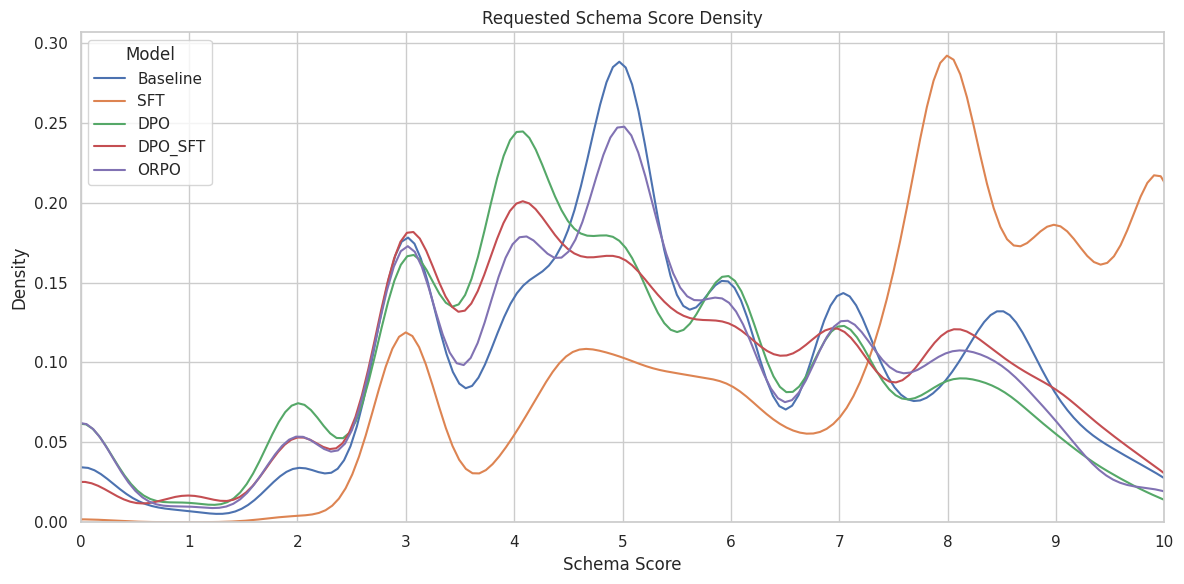
\includegraphics[width=0.9\textwidth]{images/density.png}
    \captionof{figure}{Density of the scores of the requested schema}
    \label{fig:score_distribution}
\end{strip}


\subsection{Schema Analysis}
In the following section, we will look at the individual scoring for each schema and analyze the tables in the Appendix \ref{sec: appendix schema analysis}.

For the questions related to the requested \textit{Analogy} (Table~\ref{tab: analogy}), no model managed to outperform the baseline of $55.4\%$ in terms of schema alignment, with the SFT second with $53.2\%$. In line with the overall score, the ORPO has the highest context alignment with $73.1\%$. In addition to ORPOs $35.4\%$, SFT beats the baseline when considering schema and context, with a marginal increase from $30.1\%$ to $32.3\%$.

From Table \ref{tab: cause to effect} we see that SFT completely excels in the \textit{Cause to Effect} schema with $79\%$, beating the baseline of $20.4\%$ by a long shot. ORPO is the worst model here with $15.5\%$. DPO with SFT ($80.1\%$) and ORPO ($79.1\%$) perform best in context. Although SFT is the worst in context ($58.6\%$), when considering context and scheme, it performs best with $43.5\%$ over the $12.9\%$ baseline.

$44.1\%$ of the questions in the \textit{Expert Opinion} schema generated by the baseline are critical (Table~\ref{tab: expert opinion}). SFT significantly increased this to $97.3\%$, while the second-best, DPO with SFT, only manages $51.6\%$. In terms of context, all models beat the baseline of $60.2\%$, and the standard DPO gained the highest with $69.4\%$. Being the only one to increase the baseline's $22\%$ by more than $250\%$ to $60.8\%$, the SFT performs best when considering both the context and the schema alignment. 

The \textit{Fear-Appeal} schema struggled the most, with the SFT being the highest by a large margin, $31.7\%$ above the baselines $7.5\%$ (Table~\ref{tab: fear appeal}). In terms of context, it is similar to the others, with ORPO achieving $82.8\%$ and increasing the baselines $69.9\%$ the most. When both are combined, SFT remains at the top with $14.5\%$. This beats the baseline of $5.9\%$. 

For the first 3 schemas, SFT was the only model to consistently achieve its average and median to meet the threshold of 7. Sometimes, it came at the cost of a high standard deviation, which was maximized at $2.09$. The only other two models to obtain a median above the threshold are the baseline for \textit{Analogy} with $7.25$ and DPO with SFT in \textit{Expert Opinion} with $7.00$. Furthermore, it is also worth noting that none of the models has an average or median that meets the critical threshold of 7 in the schema \textit{Fear-Appeal}, with SFT achieving the highest (5.49 and 5.00). To visualize the distributions of each schema, we refer to the Appendix \ref{sub: distribution of schema score}.
\begin{table} [H]
    \centering
    \begin{tabular}{p{1.4cm}p{2cm}p{2cm}}
        \hline
        \textbf{Model} & \textbf{multiple schema critical} & \textbf{additional schema critical}\\
        \hline
Baseline        &	77  & 72 \\
SFT	            &   \textbf{216} & \textbf{202}\\
DPO	            &   59 & 48\\
DPO with SFT	&   83 & 70\\
ORPO            &   78 & 65 \\
        \hline
    \end{tabular}
    \caption{Evaluation Multi-schema criticality}
    \label{tab: multi}
\end{table}

Moving on, we see from Table \ref{tab: multi} how many of the questions generated from each model fulfill multiple schemas. $27.15\%$ of SFT's questions are of more than 1 schema. In addition to that, 202 of the 486 ($41.56\%$) of the critical questions are also critical in one more schema. The other models align more with the baseline, where only 72 of 237 ($30.38\%$) critical questions have an additional schema. The standard DPO generates the fewest questions that satisfy an additional schema. 

Regarding the questions that fulfill a schema but not the requested one, we look at Table \ref{tab: other}. SFT managed to perform best, with 103 of the 744 ($13.84\%$) generated questions being critical but in the wrong schema. ORPO's $18.95\%$ is the only model to have a higher confusion than the baseline's $18.41\%$.

\begin{table} [H]
    \centering
    \begin{tabular}{ll}
        \hline
        \textbf{Model} & \textbf{Critical in wrong schema}\\
        \hline
Baseline        &	137  \\
SFT	            &   \textbf{103}\\
DPO	            &   118    \\
DPO with SFT	&   130   \\
ORPO            &   105   \\
        \hline
    \end{tabular}
    \caption{Evaluation on wrong schema}
    \label{tab: other}
\end{table}

This can be further observed in the confusion matrices in the appendix \ref{sub: confusion matrices}. Important to note is that, with confusion, we mean that a generated question is not achieving the highest schema score in its requested schema. This does not mean that the question automatically does not satisfy the schema. In general, they show that the \textit{Expert Opinion} schema has the least confusion with other schemas. The confusion for \textit{Expert Opinion} is minimized in SFT, where 183 of the 186 ($98.39\%$) requested questions have the highest score in the requested schema. With 172 of the 186 ($92.47\%$), \textit{Cause to Effect} confusion is also the lowest in SFT. The other models struggle in \textit{Cause to Effect} with \textit{Fear-Appeal} and \textit{Analogy}, reaching $22.58\%$ and $36.6\%$ of the requested schema being of the other schema. In general, all models have similar confusions when it comes to \textit{Fear-Appeal} and \textit{Analogy}. \textit{Fear-Appeal} struggles the most in all models, with at least $54.3\%$ of the questions generated aligning more with \textit{Cause to Effect}, and at least $18.82\%$ with \textit{Analogy}. Therefore, only $18.28\%$ of the generated \textit{Fear-Appeal} questions have the correct schema as their highest score. \textit{Analogy}, as the last schema, is similar to \textit{Fear-Appeal} and has its highest confusion with up to 110 of the 186 ($59.14\%$) with \textit{Cause to Effect}. In contrast to \textit{Fear-Appeal}, up to $45.7\%$ of the questions have the requested schema as the highest score.

\subsection{Example Questions}
For this part of the analysis, we will briefly examine questions generated for the same input. DPO is not considered here, since DPO with SFT surpasses it in close to all metrics. The entire input can be found in the Appendix \ref{sec: question comparison}.
\begin{table} [H]
    \centering
    \begin{tabular}{p{1.4cm}p{5.5cm}}
    \hline
    \textbf{Model} & \textbf{question}\\
    \hline
     Baseline & Does increased cooperation with the American Muslim community, as a result of Clinton's proposed policies, effectively reduce the likelihood of terrorist attacks in the US?\\
     SFT & What if the lack of close working cooperation with Muslim nations and the American Muslim community causes their intelligence benefits to manifest and affect their ability to effectively counter terrorism? \\
     DPO with SFT & Could the close working cooperation with Muslim nations and the American Muslim community be more effective in providing intelligence if Donald's rhetoric did not alienate and push them away?\\
     ORPO & Does close cooperation with Muslim nations and the American Muslim community actually yield more intelligence benefits than cooperation with non-Muslim nations and communities? \\
    \end{tabular}
    \caption{\textit{Cause To Effect} generated questions for the same input.}
    \label{tab: example generated questions cause}
\end{table}
For \textit{Cause to Effect}, we see all four models aiming at the same question, just phrased differently (Table \ref{tab: example generated questions cause}). ORPO performs the worst (score of 0), not achieving a comparative question that aligns with the structure of a \textit{Cause to Effect} and generating more of a factual inquiry rather than a critical question. The best is from DPO with SFT (score of 8.5), which contains a clear structure, multi-layered causality, and even implicit comparison. SFT (score of 7.5) also performs well with counterfactual framing ("What if"). The baseline score is 4 and directly connects a cause with an effect. From a human perspective, it can be perceived as a critical question, but compared to the SFT and DPO with SFT it could lack depth by staying on a surface level.

\begin{table} [H]
    \centering
    \begin{tabular}{p{1.4cm}p{5.5cm}}
    \hline
    \textbf{Model} & \textbf{question}\\
    \hline
     Baseline & Does any credible intelligence agency support the claim that working closely with Muslim-majority nations and the American Muslim community yields a significant increase in intelligence gathering? \\
     SFT & Do you have any scientific source that supports the claim that working with Muslim nations and the American Muslim community is an intelligence benefit, as opposed to just a hypothetical claim? \\
     DPO with SFT & Can you provide evidence that Donald's dismissive attitude towards Muslim nations and communities has led to increased cooperation and intelligence sharing from these regions? \\
     ORPO & Can you provide evidence from your experience working with NATO and Muslim-majority nations that suggests their cooperation with the US is more effective under Democratic leadership than under Republican leadership?\\
    \end{tabular}
    \caption{\textit{Expert Opinion} generated questions for the same input.}
    \label{tab: example generated questions expert}
\end{table}

In terms of \textit{Expert Opinion}, we see in Table \ref{tab: example generated questions expert} the baseline (score 4) that challenges the intelligence agency as an external authority, asking for evidence. SFT (score 8) improves on this by asking for empirical justification and highlights the belief as a hypothesis, directly challenging the assumption. It also applies better scientific framing and a higher epistemic pressure. DPO with SFT (score 4) asks for evidence, but rather misaligns with the schema by not really seeking expert validation. In addition, it comes across as sarcastic in suggesting a positive effect from a negative cause. ORPO (score 7) is good at directly appealing to expert experiences ("from your experience") in a comparative approach. The only thing that can be framed as a drawback is that it is more anecdotal than empirical.

Table \ref{tab: example generated questions analogy} shows the \textit{Analogy} generations. While baseline (score 7.5) and SFT (score 8.5) have good analogy clarity, DPO with SFT (score 4.5) blurs this into a rhetorical contraction, and ORPO just compares two political styles. Important here is the phrasing where ORPO just asks "if A, why not B" and not "A is more like B", as an analogy would suggest. We also see here that the trained models seem to have a common conditional structure ("if"). 

\begin{table} [H]
    \centering
    \begin{tabular}{p{1.4cm}p{5.5cm}}
    \hline
    \textbf{Model} & \textbf{question}\\
    \hline
     Baseline & Would prioritizing cooperation with Muslim nations and communities be seen as a more effective counter-terrorism strategy than alienating them through rhetoric?\\
     SFT & If so, would the cooperation with Muslim nations and the American Muslim community be seen as an intelligence benefit if they are consistently alienated and pushed away by the rhetoric of a leader?\\
     DPO with SFT & If we're seeking intelligence from Muslim-majority nations and communities, does that not undermine the very rhetoric that Donald has used to alienate and push away the American Muslim community?\\
     ORPO & If working closely with Muslim nations to gather intelligence is crucial in combating terrorism, why should we assume that Donald Trump's dismissive approach towards Muslims would be any less effective than Clinton's inclusive approach? \\
    \end{tabular}
    \caption{\textit{Analogy} generated questions for the same input.}
    \label{tab: example generated questions analogy}
\end{table}

The generated questions for \textit{Fear-Appeal} align with the struggles we observed in the quantitative results, where we see the four struggling to generate a question that aligns with the schema (Table \ref{tab: example generated questions fear}). DPO with SFT (score 4) manages to have a fear element by an implicit fear of data loss. It still suffers from the same issues as the other models, with a lack of urgency or risk that is needed for the appeal of fear to apply.

\begin{table} [H]
    \centering
    \begin{tabular}{p{1.4cm}p{5.5cm}}
    \hline
    \textbf{Model} & \textbf{question}\\
    \hline
     Baseline & If working closely with Muslim nations and the American Muslim community is crucial for intelligence gathering, then why has Donald's rhetoric alienated them and undermined that cooperation?\\
     SFT & If we're working closely with Muslim nations and the American Muslim community to combat terrorism, then why does Donald's rhetoric towards Muslims, both abroad and at home, seem to be counterproductive to this effort?\\
     DPO with SFT & If the American Muslim community can provide valuable intelligence to counter terrorism, why does Donald's rhetoric towards them continue to be alienating and push them away? \\
     ORPO & Does the effectiveness of intelligence gathering from Muslim-majority nations justify the potential risks associated with alienating them due to Donald's rhetoric?\\
    \end{tabular}
    \caption{\textit{Fear-Appeal} generated questions for the same input.}
    \label{tab: example generated questions fear}
\end{table}

\section{Discussion}

The evaluation results underscore the capabilities and improvements that arise through fine-tuning for critical question generation. Of all the models, Supervised Fine-Tuning (SFT) showed the strongest performance, especially excelling in schema alignment, achieving $65.3\%$  criticality and more than double the baseline. The greatest alignment gains were made with the \textit{Expert Opinion} schema, reaching $97.3\%$, and similar gains were observed for \textit{Cause to Effect}. These findings suggest that the approach of the paper using schema-specific training data enables models to grasp the underlying structure of different argumentative schemas.  
 
The Reinforcement Learning approaches, such as DPO and ORPO, showed a more mixed result. Despite their improvements in context alignment, they underperformed in generating structurally critical questions.
For example, ORPO achieved the highest overall context alignment ($75.9\%$) but scored below SFT in schema criticality. But if the goal is to succeed in the evaluation of the original Shared Task challenge, ORPO improves the most with $78.2\%$, beating the baseline's $69.8\%$. This difference in the results of the two evaluation approaches raises the question of whether the project was focused on the right one. The original task labels the questions on the basis of their similarity to the preselected questions. This has an inherent flaw in not being able to assess questions that were not previously considered. They circumvented this by providing the schema on which the pre-selected questions align, so only questions in these schemas are generated. The approaches presented in this paper overcame this limitation with a generalized approach that treats semantics and syntax separately, without the need for previous expert analysis. This allows a broader application of the model and should allow more data to be included easily.

The schema-specific analysis offers further insight into the complexity of this task. SFT performed best in all schemas, but significant performance disparities were observed between them. Structurally explicit schemas, such as \textit{Cause to Effect} and \textit{Expert Opinion}, were easier for models to learn. Specifically, \textit{Cause to Effect} (up to $43.5\%$ accuracy) dominated more niche schemas, like \textit{Fear-Appeal} (up to $14.5\%$ accuracy), which often involved implicit emotional or rhetorical cues. This originates from the fact that not all inputs provide the content for the schema, making it impossible to generate satisfying questions. But even if it is possible, the subjective matter of the degree of fear appeal is shown in the example questions, where the lack of severity and urgency crystallizes. This suggests that not all critical question types are equally learnable, particularly when evaluation is based on rigid structural heuristics, and schemas contain subjective nuances.

Another interesting finding concerns the multi-schema alignment exhibited by the SFT model. More than $27\%$ of its questions were aligned with more than one argumentation scheme, indicating a capacity to generate complex, multifaceted questions. However, this flexibility also introduced confusion, particularly between semantically adjacent schemas such as \textit{Analogy} and \textit{Cause to Effect}. This is further confirmed through the analyzed example questions, which show the trend to include causation in other schema questions. Although this ambiguity can be seen as a feature in certain contexts, it complicates schema-specific evaluation and may hinder downstream applications that require precise argumentative structures.

\subsection{Limitations}
Despite these advances, several limitations remain with this approach. The first and most obvious one is the constrained schema coverage. Only four of Walton’s 18 argumentation schemes were implemented, limiting the generalizability of the approach. Although these four were chosen for their clarity and prevalence, excluding broader classes such as \textit{Argument from Sign} or \textit{Argument from Consequences} narrows the ability of the model to reflect the full range of critical inquiry present in real discourse.

Secondly, the quality and origin of the training data pose another constraint. The data set provides questions, but most of the questions are not necessarily critical to our application. This limitation is compounded by an inherent domain bias toward political or philosophical discourse, which further restricts generalizability. An ideal data set would have equal representations of each schema in different domains and tones. To this comes the issue of multi-schema questions in the training set, which introduces potential confusion in understanding the underlying schema. For reinforcement learning approaches, it is also important to have quality data on rejected questions, highlighting the differences between the schemas. 

Another key limitation is the rigidity of the evaluation framework itself. Although the rule-based scoring system ensures consistency and scalability, it may not cover all aspects of the schema. This leads to rejecting potential critical questions that were not previously considered. In particular, in the case of more subjective or emotionally nuanced schemas, such as \textit{Fear-Appeal}, the current system struggles to capture the full intent behind a question. Extending this is a future work limitation in overcoming the schema and context alignment disparity, as observed in the results.

\subsection{Future Work}
To overcome these limitations, several directions can be pursued in future research. One priority is to expand the schema coverage beyond the initial four categories. Expanding the set of linguistic and argumentation schemes beyond the four currently used would also allow for a more comprehensive and nuanced treatment of argumentative structures, supporting a broader range of critical inquiries. By encompassing all the schemas used in the validation set, an improvement in the shared task challenge is almost guaranteed.

Another crucial step is the development of a dedicated data set for the generation of critical questions. The data set should be explicitly annotated with Walton's argumentation schemes and criticality labels. Ideally, it would span multiple domains and include a range of rhetorical styles, from formal reasoning to emotionally charged discourse. This would enable models to learn not only structural patterns but also the pragmatic aspects of questioning in argumentative dialogue.

The evaluation framework itself also requires an improvement. The scoring system should be reviewed in cooperation with experts in the linguistic field to ensure completeness and an expert view of the rules-based heuristics. Future iterations could also incorporate a hybrid scoring approach that combines rule-based heuristics with human-in-the-loop validation. This would enable the system to capture not just structural fidelity but also perceived effectiveness and impact. Moreover, employing dynamic schema prediction, where models first infer the most appropriate schema before generating a question, could reduce confusion and improve performance in multischema contexts.

Finally, more advanced reinforcement learning techniques with improved reward functions would be a more complex and potentially insightful approach. Our current approach does not directly consider the scoring in the schema, only labeling questions as critical in a schema. By including the scores of each question in the training, we assume that the confusion can be reduced and the capture of the inherent structure of a schema is improved. This can also be further extended by incorporating the specific criteria that a question fulfills to enrich the data with as much information as possible. This would be a step forward from the current proof-of-concept, which would lead to a promising model. 

\newpage
% Entries for the custom entries
\bibliography{custom}
\bibliographystyle{acl_natbib}

\appendix
\onecolumn
\section{Appendix}
\label{sec:appendix}
\subsection{Schema analysis}
\label{sec: appendix schema analysis}

\begin{table}[H]
    \centering
    \begin{tabular}{lllllll}
        \hline
        \textbf{Model} & \textbf{Average} & \textbf{Median} & \textbf{Std Dev} & \textbf{\% Critical} &  \textbf{\% in Context} & \textbf{\% in Context \& Critical} \\
        \hline
        Baseline & 6.69 & 7.25 & 1.87 & \textbf{55.4} & 58.1 & 30.1 \\
        SFT & \textbf{7.11} & \textbf{7.50} & 2.09 & 53.2 & 66.7 & 32.3 \\
        DPO & 5.73 & 5.00 & 1.81 & 32.8 & 70.4 & 24.2 \\
        DPO with SFT & 6.01 & 5.50 & 1.82 & 33.3 & 71.5 & 23.7 \\
        ORPO & 6.37 & 5.50 & \textbf{1.76} & 45.7 & \textbf{73.1} & \textbf{35.5} \\
        \hline
    \end{tabular}
    \caption{\textit{Analogy} evaluation}
    \label{tab: analogy}
\end{table}

\begin{table}[H]
    \centering
    \begin{tabular}{lllllll}
        \hline
        \textbf{Model} & \textbf{Average} & \textbf{Median} & \textbf{Std Dev} & \textbf{\% Critical} &  \textbf{\% in Context} & \textbf{\% in Context \& Critical} \\
        \hline
        Baseline & 5.21 &	5.00 &	2.45 &	20.4 &	65.6 &	12.9\\
        SFT & \textbf{7.81} &	\textbf{8.00} &	\textbf{1.65} &	\textbf{79.0} &	58.6 &	\textbf{43.5} \\
        DPO & 4.58 &	4.00 & 2.71 &	22.6 &	72.6 &	16.1 \\
        DPO with SFT & 5.19 & 5.00 & 2.72 & 28.5 & \textbf{80.1} &	21.0 \\
        ORPO & 4.16 & 4.75 & 2.82 & 15.6 & 79.6 & 12.4 \\
        \hline
    \end{tabular}
    \caption{Cause to Effect evaluation}
    \label{tab: cause to effect}
\end{table}

\begin{table}[H]
    \centering
    \begin{tabular}{lllllll}
        \hline
        \textbf{Model} & \textbf{Average} & \textbf{Median} & \textbf{Std Dev} & \textbf{\% Critical} &  \textbf{\% in Context} & \textbf{\% in Context \& Critical} \\
        \hline
Baseline&	5.80&	6.00&	2.08	&44.1&	60.2&	22.0\\
SFT&	\textbf{8.72}&	\textbf{9.00}&	\textbf{1.03}&	\textbf{97.3}&	61.8&	\textbf{60.8}\\
DPO&	5.40&	6.00&	2.40&	38.2&	\textbf{69.4}&	28.0\\
DPO with SFT &	6.12&	7.00	&2.30	&51.6&	66.1&	30.1 \\
ORPO & 5.93 & 6.00 & 1.89 & 44.1 & 68.3 & 29.6 \\
        \hline
    \end{tabular}
    \caption{\textit{Expert Opinion} evaluation}
    \label{tab: expert opinion}
\end{table}

\begin{table}[H]
    \centering
    \begin{tabular}{lllllll}
        \hline
        \textbf{Model} & \textbf{Average} & \textbf{Median} & \textbf{Std Dev} & \textbf{\% Critical} &  \textbf{\% in Context} & \textbf{\% in Context \& Critical} \\
        \hline
Baseline&	4.25&	4.00	&\textbf{1.51}&	7.5&	69.9&	5.9\\
SFT	&\textbf{5.49}	&\textbf{5.00}&	2.42	&\textbf{31.7} &	75.3&	\textbf{14.5}\\
DPO	&4.15	&4.00&	1.52	&5.9&	75.8&	4.3\\
DPO with SFT	&4.28&	4.00	&1.60	&9.7&	75.8&	8.1 \\
ORPO & 4.23 & 4.00 & 1.53 & 7.5 & \textbf{82.8} & 5.4 \\
        \hline
    \end{tabular}
    \caption{\textit{Fear-Appeal} evaluation}
    \label{tab: fear appeal}
\end{table}

\subsection{Distribution of scores for each Schema}
\label{sub: distribution of schema score}
\begin{figure}[H]
  \centering
  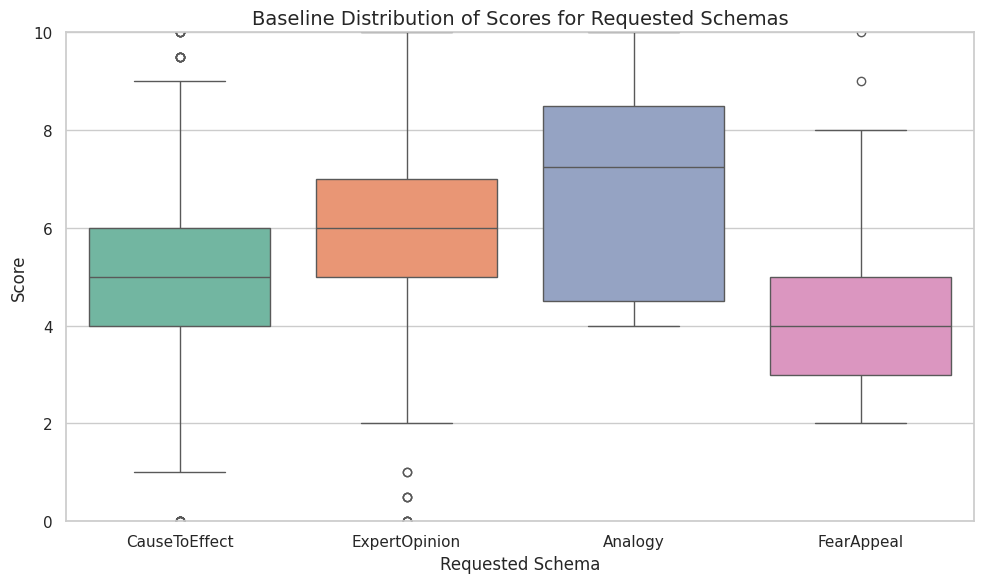
\includegraphics[width=0.7\textwidth]{images/base_dis.png}
    \caption{Baseline}
\end{figure}
\begin{figure}[H]
  \centering
  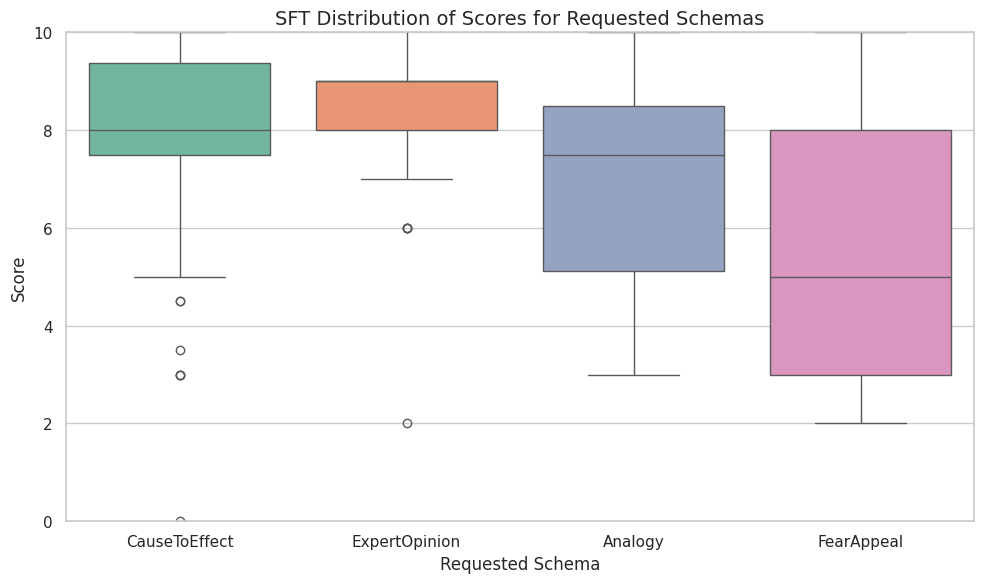
\includegraphics[width=0.7\textwidth]{images/sft_dis.png}
    \caption{SFT}
\end{figure}
\begin{figure}[H]
  \centering
  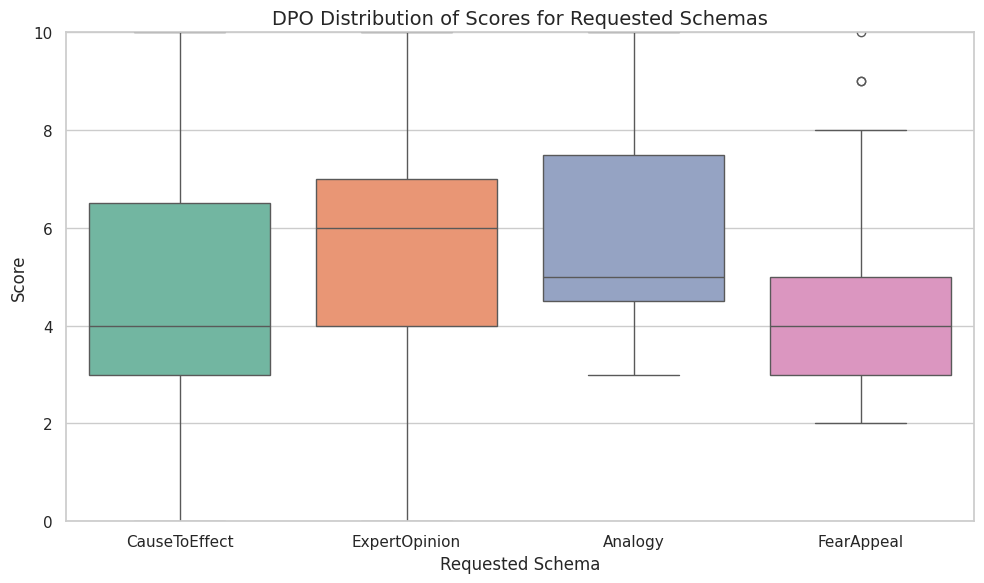
\includegraphics[width=0.7\textwidth]{images/dpo_dis.png}
    \caption{DPO}
\end{figure}
\begin{figure}[H]
  \centering
  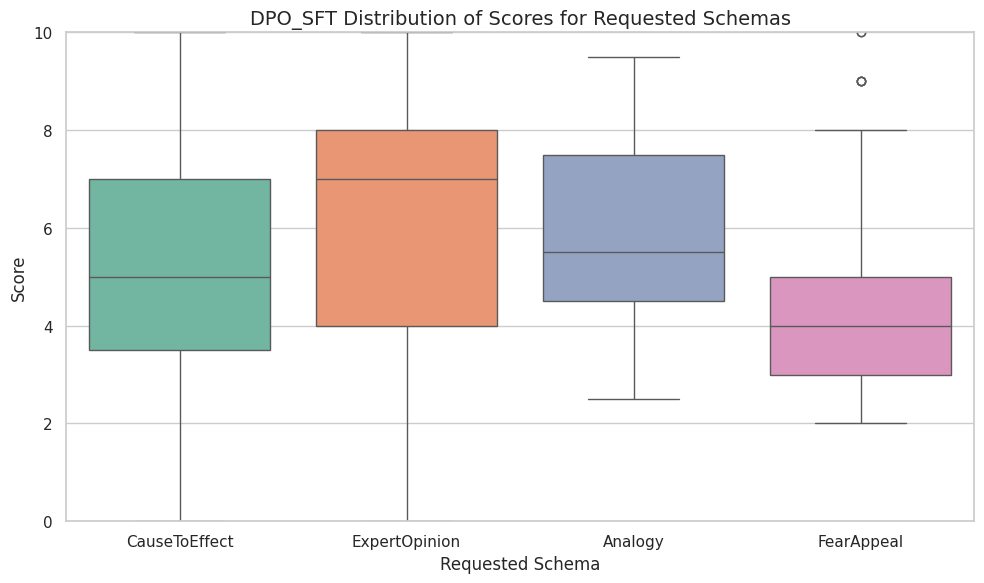
\includegraphics[width=0.7\textwidth]{images/dpo_sft_dis.png}
    \caption{DPO with SFT}
\end{figure}
\begin{figure}[H]
  \centering
  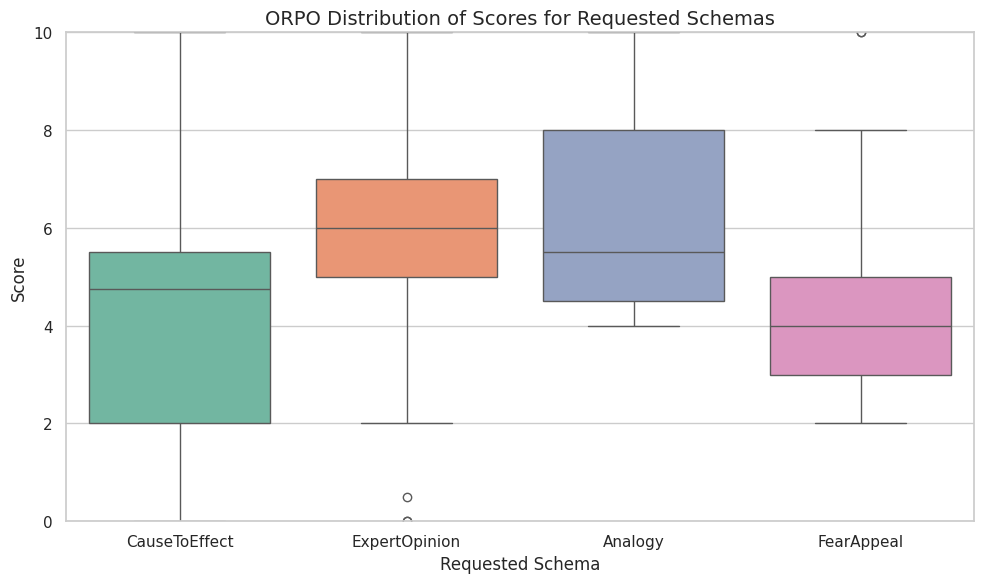
\includegraphics[width=0.7\textwidth]{images/orpo_dis.png}
    \caption{ORPO}
\end{figure}

\subsection{Confusion Matrices}
\label{sub: confusion matrices}
\begin{figure}[H]
  \centering
  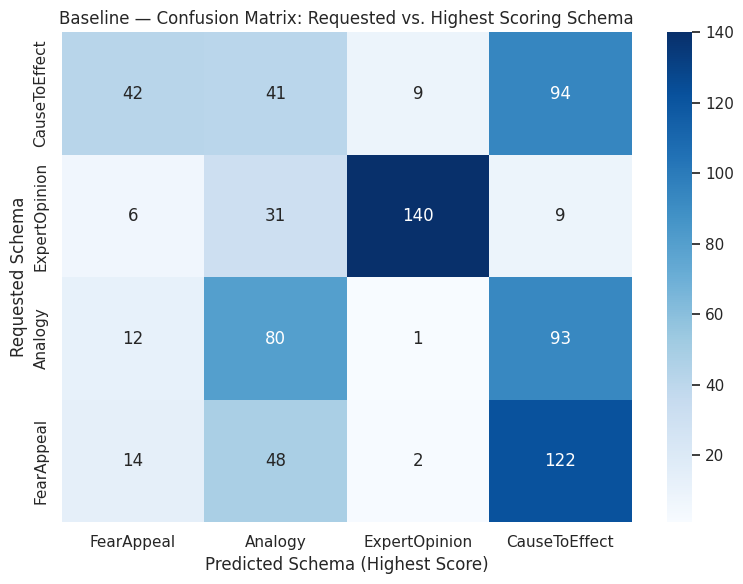
\includegraphics[width=0.8\textwidth]{images/base_conf.png}
    \caption{Baseline}
\end{figure}
\begin{figure}[H]
  \centering
  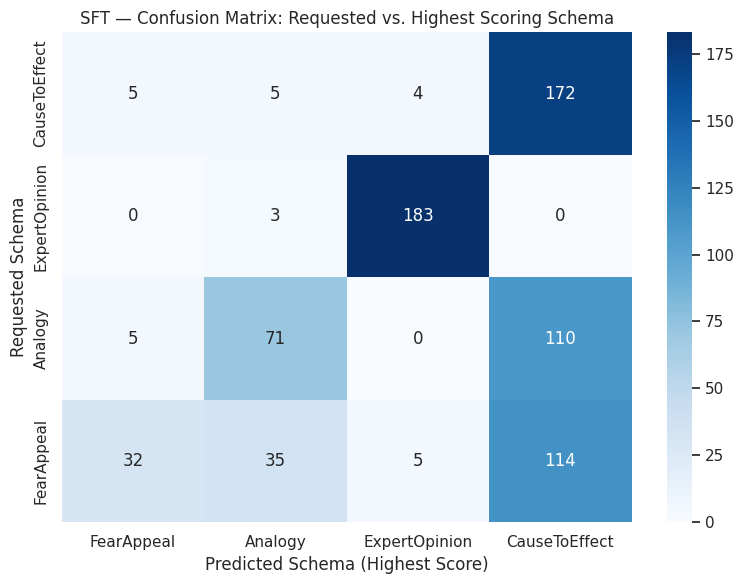
\includegraphics[width=0.8\textwidth]{images/sft_conf.png}
    \caption{SFT}
\end{figure}
\begin{figure}[H]
  \centering
  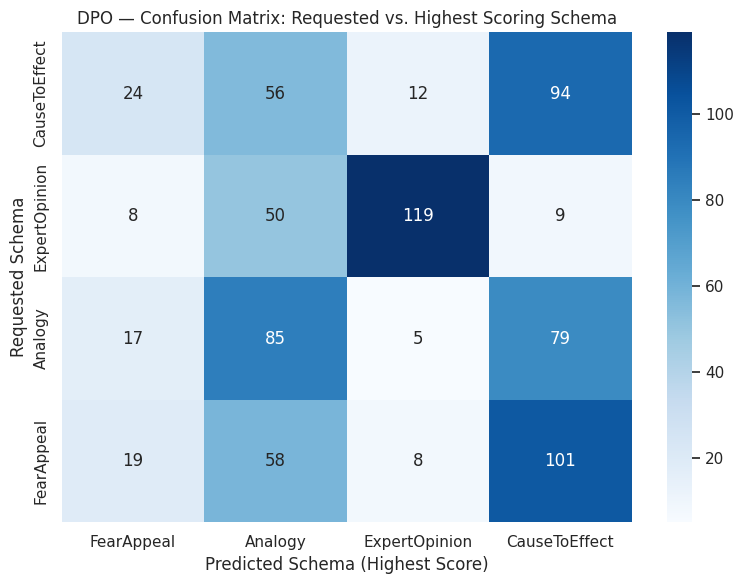
\includegraphics[width=0.8\textwidth]{images/dpo_conf.png}
    \caption{DPO}
\end{figure}
\begin{figure}[H]
  \centering
  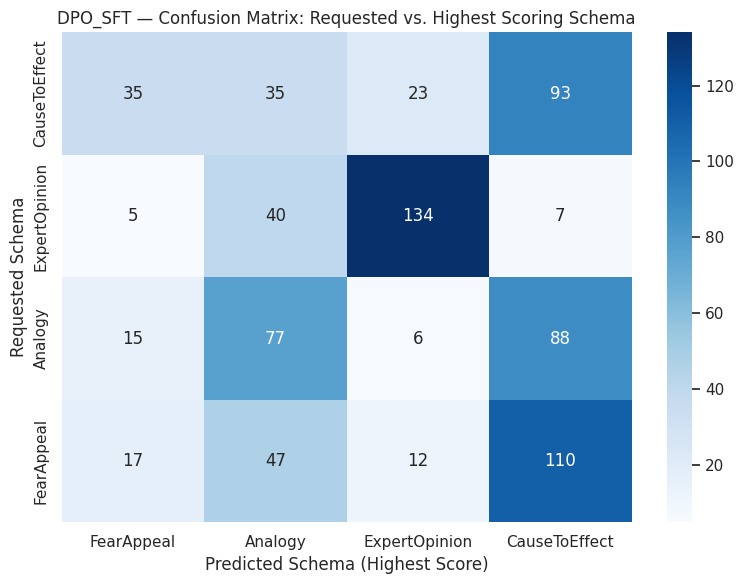
\includegraphics[width=0.8\textwidth]{images/dpo_sft_conf.png}
    \caption{DPO with SFT}
\end{figure}
\begin{figure}[H]
  \centering
  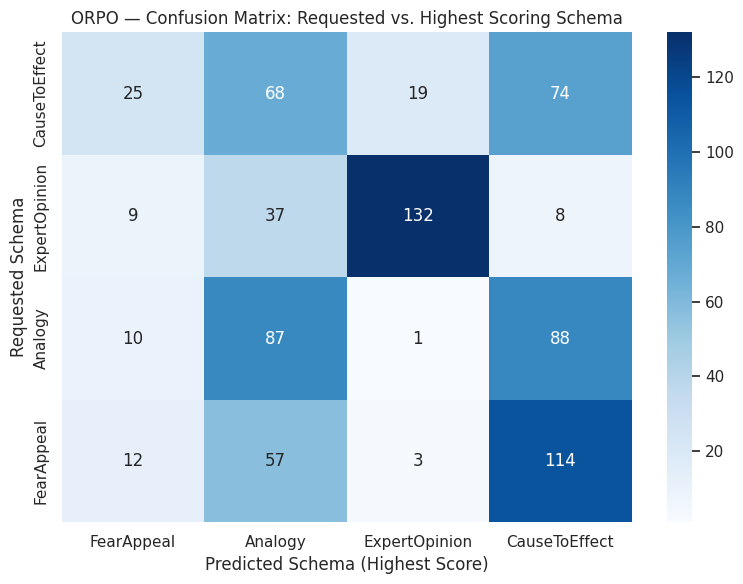
\includegraphics[width=0.8\textwidth]{images/orpo_conf.png}
    \caption{ORPO}
\end{figure}

\subsection{Templates of Critical Questions from Walton's Theory}
\begin{table} [H]
\centering
\begin{tabular}{p{4cm}p{12cm}}
\hline
\textbf{Argumentation Scheme} & \textbf{Example Questions} \\
\hline
Argument from Expert Opinion & Is <expertE> a genuine expert in <domainD>? Did <expertE> really assert that <eventA>? 

Is <expertE>'s pronouncement directly quoted? If not, is a reference to the original source given? 

Can it be checked? 

If <expertE>'s advice is not quoted, does it look like important information or qualifications may have been left out? 

Is what <expertE> said clear? Are there technical terms used that are not explained clearly? 

Is <eventA> relevant to domain <domainD>? 

Is <eventA> consistent with what other experts in <domainD> say? Is <eventA> consistent with known evidence in <domainD>? \\
\hline
Argument from Cause to Effect & How strong is the generalisation that if <eventA> then <eventB>? 

Are there other factors in this particular case that could have interfered with the event of <eventB>? \\
\hline
Argument from Analogy & Are <C1> and <C2> similar in the respect cited?

Is <eventA> true in <C1>? 

Are there differences between <C1> and <C2> that would tend to undermine the force of the similarity cited? 

Is there some other case that is also similar to <C1>, but in which <eventA> is false? \\
\hline
Argument from Danger Appeal & If <eventA>, will <eventB> occur?

What evidence supports this claim?

Why is <eventB> a danger? To whom is <eventB> a danger?

Is there a way of preventing <eventA>?

Are there other consequences of preventing <eventA> that we should take into account? \\
\hline
\end{tabular}
\caption{Templates of Critical Questions from Argumentation Theory}
\label{tab:argumentation_questions}
\end{table}

\subsection{Model question comparison}
\label{sec: question comparison}
Input of CLINTON\_199\_2:


CLINTON: which may prove to be an intelligence benefit. We've got to do everything we can to vacuum up intelligence from Europe, from the Middle East. That means we've got to work more closely with our allies, and that's something that Donald has been very dismissive of. We're working with NATO, the longest military alliance in the history of the world, to really turn our attention to terrorism. We're working with our friends in the Middle East, many of which, as you know, are Muslim majority nations. Donald has consistently insulted Muslims abroad, Muslims at home, when we need to be cooperating with Muslim nations and with the American Muslim community. They're on the front lines. They can provide information to us that we might not get anywhere else. They need to have close working cooperation with law enforcement in these communities, not be alienated and pushed away as some of Donald's rhetoric, unfortunately, has led to

\end{document}
